\hypertarget{newConv_8c}{
\section{new\-Conv.c File Reference}
\label{newConv_8c}\index{newConv.c@{newConv.c}}
}
{\tt \#include \char`\"{}bit\-Set.h\char`\"{}}\par
{\tt \#include $<$errno.h$>$}\par
{\tt \#include \char`\"{}convll.h\char`\"{}}\par


Include dependency graph for new\-Conv.c:\begin{figure}[H]
\begin{center}
\leavevmode
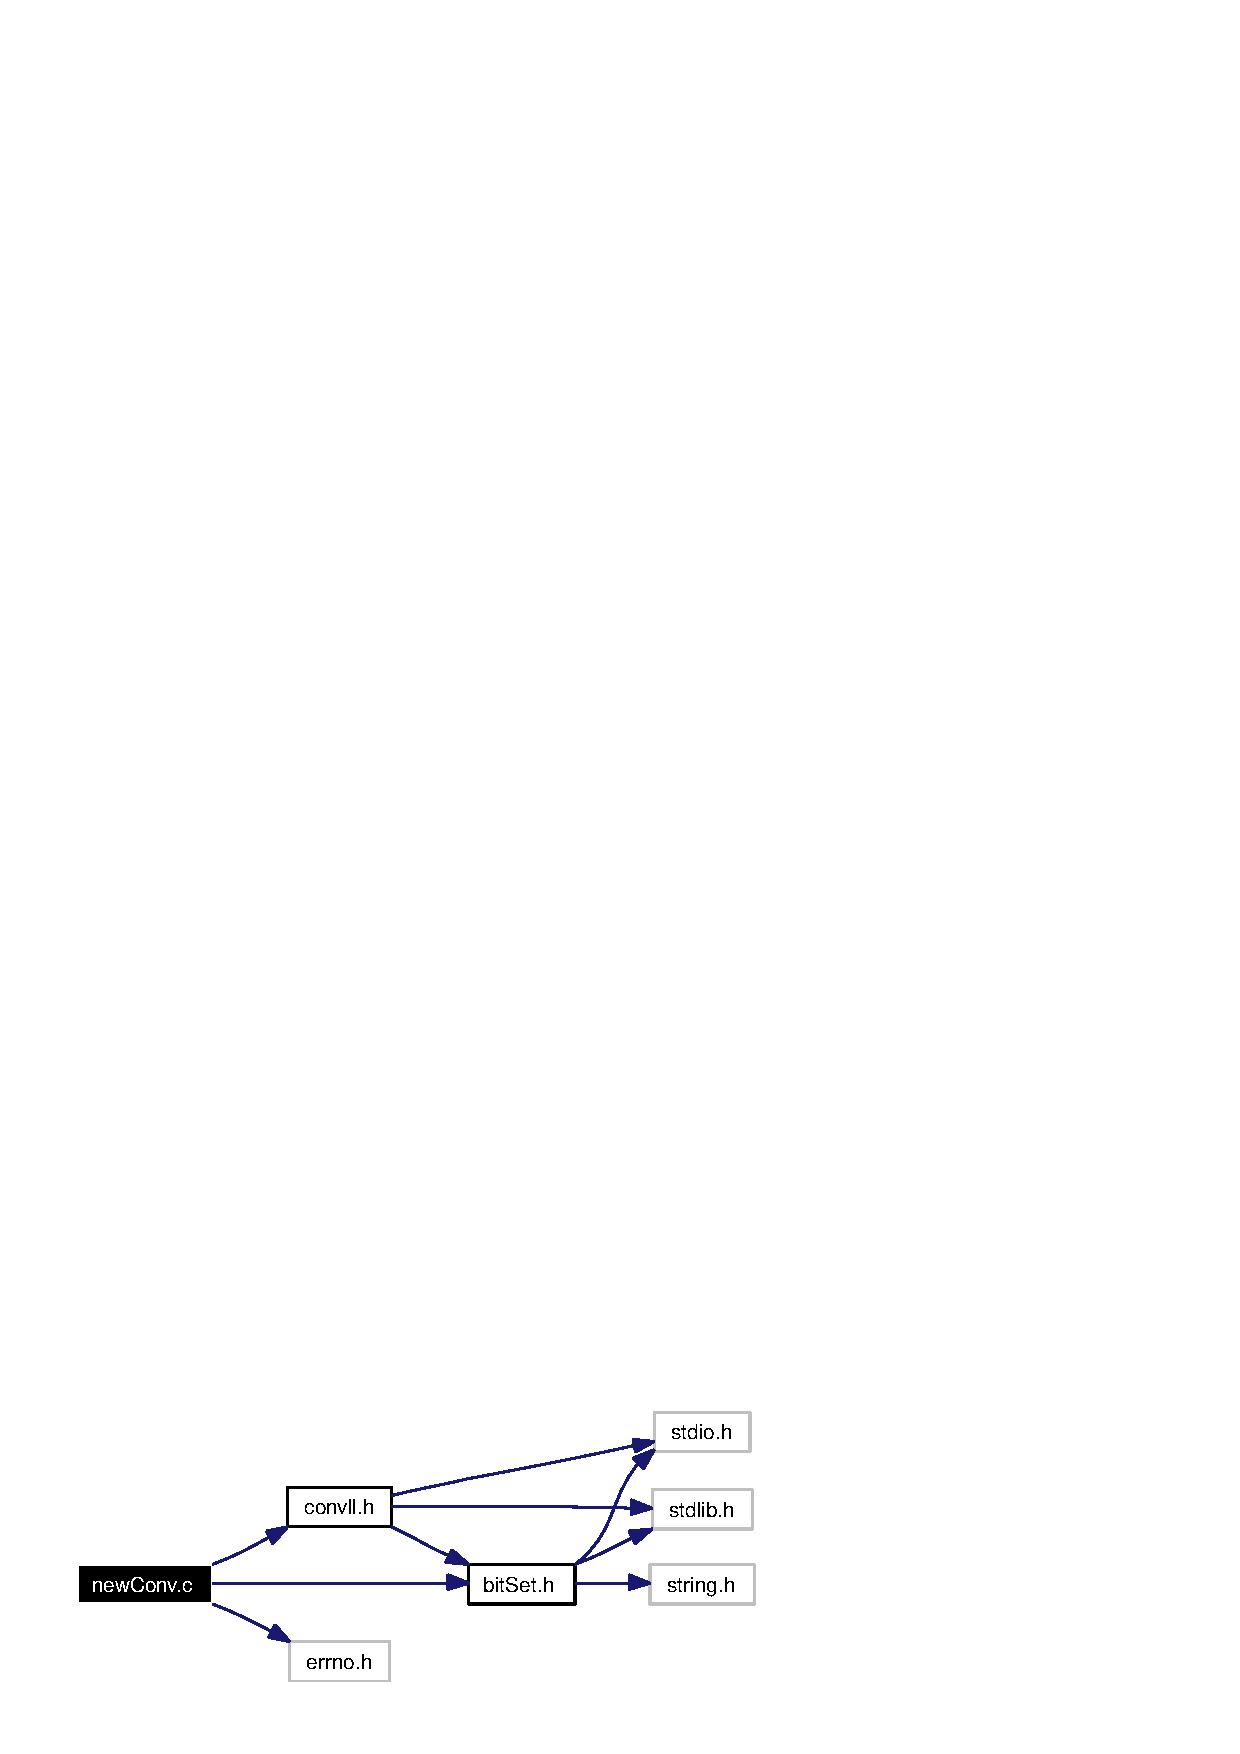
\includegraphics[width=181pt]{newConv_8c__incl}
\end{center}
\end{figure}
\subsection*{Functions}
\begin{CompactItemize}
\item 
int \hyperlink{newConv_8c_a0}{find\-Cliques} (\hyperlink{structbitSet__t}{bit\-Set\_\-t} $\ast$Q, \hyperlink{structbitSet__t}{bit\-Set\_\-t} $\ast$cand, \hyperlink{structbitSet__t}{bit\-Set\_\-t} $\ast$mask, \hyperlink{structbitGraph__t}{bit\-Graph\_\-t} $\ast$o\-G, int support, int q\-Count, \hyperlink{structcnode}{cll\_\-t} $\ast$$\ast$elem\-Pats, int $\ast$index\-To\-Seq, int p)
\item 
int \hyperlink{newConv_8c_a1}{single\-Linkage} (\hyperlink{structbitSet__t}{bit\-Set\_\-t} $\ast$Q, \hyperlink{structbitSet__t}{bit\-Set\_\-t} $\ast$cand, \hyperlink{structbitSet__t}{bit\-Set\_\-t} $\ast$mask, \hyperlink{structbitGraph__t}{bit\-Graph\_\-t} $\ast$o\-G, int support, int q\-Count, \hyperlink{structcnode}{cll\_\-t} $\ast$$\ast$elem\-Pats, int $\ast$index\-To\-Seq, int p)
\item 
int \hyperlink{newConv_8c_a2}{filter\-Iter} (\hyperlink{structbitGraph__t}{bit\-Graph\_\-t} $\ast$graph, int support, \hyperlink{structbitSet__t}{bit\-Set\_\-t} $\ast$changed, \hyperlink{structbitSet__t}{bit\-Set\_\-t} $\ast$work)
\item 
int \hyperlink{newConv_8c_a3}{filter\-Graph} (\hyperlink{structbitGraph__t}{bit\-Graph\_\-t} $\ast$graph, int support, int R)
\item 
\hyperlink{structbitGraph__t}{bit\-Graph\_\-t} $\ast$ \hyperlink{newConv_8c_a4}{prune\-Bit\-Graph} (\hyperlink{structbitGraph__t}{bit\-Graph\_\-t} $\ast$bg, int $\ast$index\-To\-Seq, int $\ast$$\ast$offset\-To\-Index, int num\-Of\-Seqs, int p)
\item 
\hyperlink{structcnode}{cll\_\-t} $\ast$ \hyperlink{newConv_8c_a5}{prune\-Cll} (\hyperlink{structcnode}{cll\_\-t} $\ast$head, int $\ast$index\-To\-Seq, int p)
\item 
\hyperlink{structcnode}{cll\_\-t} $\ast$ \hyperlink{newConv_8c_a6}{convolve} (\hyperlink{structbitGraph__t}{bit\-Graph\_\-t} $\ast$bg, int support, int R, int $\ast$index\-To\-Seq, int p, int cluster\-Method, int $\ast$$\ast$offset\-To\-Index, int number\-Of\-Sequences, int no\-Convolve, FILE $\ast$OUTPUT\_\-FILE)
\end{CompactItemize}


\subsection*{Detailed Description}
This file contains the core functions that performed the convolution in the Gemoda algorithm. As well, there are two clustering functions defined in this file: one for single linkage clustering, and one for clique based clustering.

Definition in file \hyperlink{newConv_8c-source}{new\-Conv.c}.

\subsection*{Function Documentation}
\hypertarget{newConv_8c_a6}{
\index{newConv.c@{new\-Conv.c}!convolve@{convolve}}
\index{convolve@{convolve}!newConv.c@{new\-Conv.c}}
\subsubsection[convolve]{\setlength{\rightskip}{0pt plus 5cm}\hyperlink{structcnode}{cll\_\-t}$\ast$ convolve (\hyperlink{structbitGraph__t}{bit\-Graph\_\-t} $\ast$ {\em bg}, int {\em support}, int {\em R}, int $\ast$ {\em index\-To\-Seq}, int {\em p}, int {\em cluster\-Method}, int $\ast$$\ast$ {\em offset\-To\-Index}, int {\em number\-Of\-Sequences}, int {\em no\-Convolve}, FILE $\ast$ {\em OUTPUT\_\-FILE})}}
\label{newConv_8c_a6}


Our outer convolution function. This function will call preliminary functions, cluster the data, and then call the main convolution function. This is the interface between the main gemoda-$<$x$>$ code and the generic code that gets all of the work done. Input: the bit\-Graph to be clustered and convolved, the minimum support necessary for a motif to be returned, a flag indicating whether recursive filtering should be used, a pointer to the data structure that dereferences offset indices to sequence numbers, the number of unique source sequences that a motif must be present in, and a number indicating the clustering method that is to be used. Output: the final motif linked list with all motifs that are to be given as output to the user.

Definition at line 625 of file new\-Conv.c.

References bit\-Graph\-Set\-False\-Diagonal(), complete\-Conv(), delete\-Bit\-Set(), fill\-Set(), filter\-Graph(), find\-Cliques(), new\-Bit\-Set(), prune\-Bit\-Graph(), prune\-Cll(), single\-Linkage(), bit\-Graph\_\-t::size, and yank\-Cll().

\scriptsize\begin{verbatim}629 {
630   bitSet_t * cand = NULL;
631   bitSet_t * mask = NULL;
632   bitSet_t * Q = NULL;
633   int size = bg->size;
634   cll_t * elemPats = NULL;
635   cll_t * allCliques = NULL;
636   cll_t * curr = NULL;
637   
638     // contains indices (rows) containing the threshold value.
639     cand = newBitSet (size);
640   mask = newBitSet (size);
641   Q = newBitSet (size);
642   fillSet (cand);
643   fillSet (mask);
644   
645     // Note that we prune based on p before setting the diagonal false.
646     if (p > 1)
647     {
648       bg =
649     pruneBitGraph (bg, indexToSeq, offsetToIndex, numberOfSequences, p);
650     }
651   
652     // Now we set the main diagonal false for clustering and filtering.
653     bitGraphSetFalseDiagonal (bg);
654   filterGraph (bg, support, R);
655   fprintf (OUTPUT_FILE, "Graph filtered!  Now clustering...\n");
656   fflush (NULL);
657   if (clusterMethod == 0)
658     {
659       findCliques (Q, cand, mask, bg, support, 0, &elemPats, indexToSeq, p);
660     }
661   else
662     {
663       singleLinkage (Q, cand, mask, bg, support, 0, &elemPats, indexToSeq,
664               p);
665     }
666   fprintf (OUTPUT_FILE,
667         "Clusters found!  Now filtering clusters (if option set)...\n");
668   fflush (NULL);
669   if (p > 1)
670     {
671       elemPats = pruneCll (elemPats, indexToSeq, p);
672     }
673   deleteBitSet (cand);
674   deleteBitSet (mask);
675   deleteBitSet (Q);
676   
677     // Now let's convolve what we made.
678     if (noConvolve == 0)
679     {
680       fprintf (OUTPUT_FILE, "Now convolving...\n");
681       fflush (NULL);
682       allCliques = completeConv (&elemPats, support, size, 0, indexToSeq, p);
683     }
684   
685   else
686     {
687       curr = elemPats;
688       while (curr != NULL)
689     {
690       yankCll (&elemPats, NULL, &curr, &allCliques, 0);
691     }
692     }
693   return allCliques;
694 }
\end{verbatim}
\normalsize 


\hypertarget{newConv_8c_a3}{
\index{newConv.c@{new\-Conv.c}!filterGraph@{filterGraph}}
\index{filterGraph@{filterGraph}!newConv.c@{new\-Conv.c}}
\subsubsection[filterGraph]{\setlength{\rightskip}{0pt plus 5cm}int filter\-Graph (\hyperlink{structbitGraph__t}{bit\-Graph\_\-t} $\ast$ {\em graph}, int {\em support}, int {\em R})}}
\label{newConv_8c_a3}


Function to \char`\"{}filter\char`\"{} the initial bit\-Graph that is being clustered. \char`\"{}Filtering\char`\"{} is the process of removing all nodes from the graph that cannot possibly be in motifs because they are not connected to enough other nodes. This can be done once (if R != 1), or it can be done recursively (if R == 1). When done recursively, it takes the just-filtered graph and checks all of the nodes that the recently removed node used to be connected to; since they have changed in connectivity, they may no longer be connected to enough nodes to be a member of a motif. This is iterated until convergence. Note that the default is to have recursive filtering on, as it ought to decrease the computational complexity of the clustering step and ought not have much of a computational footprint... in cases where it takes a while, it is probably having a good impact in the clustering step, whereas if it is not effective, it probably won't take that long anyway. Input: a bit\-Graph to be filtered, the minimum support that a motif must have, and the flag indicating recursive filtering or not. Output: Integer success value of 0 (and an altered bit\-Graph so that all nodes with connections have at least $<$min support$>$=\char`\"{}\char`\"{}$>$ connections).

Definition at line 359 of file new\-Conv.c.

References copy\-Set(), count\-Set(), delete\-Bit\-Set(), empty\-Set(), filter\-Iter(), new\-Bit\-Set(), and bit\-Graph\_\-t::size.

Referenced by convolve().

\scriptsize\begin{verbatim}360 {
361   bitSet_t * changed = newBitSet (graph->size);
362   bitSet_t * work = newBitSet (graph->size);
363   emptySet (changed);
364   emptySet (work);
365   
366     // Iteratively call the filtering by copying the previous "work" into
367     // "changed" after each iteration step.
368     if (R == 1)
369     {
370       
371       do
372     {
373       filterIter (graph, support, changed, work);
374       copySet (work, changed);
375     }
376       while (countSet (changed) > 0);
377     }
378   else
379     {
380       
381     // Otherwise, just do it once.
382     filterIter (graph, support, changed, work);
383     }
384   deleteBitSet (changed);
385   deleteBitSet (work);
386   return 0;
387 }
\end{verbatim}
\normalsize 


\hypertarget{newConv_8c_a2}{
\index{newConv.c@{new\-Conv.c}!filterIter@{filterIter}}
\index{filterIter@{filterIter}!newConv.c@{new\-Conv.c}}
\subsubsection[filterIter]{\setlength{\rightskip}{0pt plus 5cm}int filter\-Iter (\hyperlink{structbitGraph__t}{bit\-Graph\_\-t} $\ast$ {\em graph}, int {\em support}, \hyperlink{structbitSet__t}{bit\-Set\_\-t} $\ast$ {\em changed}, \hyperlink{structbitSet__t}{bit\-Set\_\-t} $\ast$ {\em work})}}
\label{newConv_8c_a2}


The iterator used to \char`\"{}filter\char`\"{} the graph. It takes information in the bitset telling which nodes' rows have changed and only checks them... this should make it pretty efficient time-wise at only a small memory cost. Note the convention that the first time this is called, the changed bit\-Set is empty... and that the master function is responsible for catching the signal that no changes were made in the last iteration. Input: the bit\-Graph to be filtered, the minimum support required for a motif to be returned, a bit\-Set with nodes changed from the previous iteration, and a bit\-Set to export the nodes changed in this iteration. Output: integer success value of 0 (and also a filtered bit\-Graph and a bit\-Set with the nodes changed in this iteration).

Definition at line 228 of file new\-Conv.c.

References count\-Set(), empty\-Set(), bit\-Graph\_\-t::graph, next\-Bit\-Bit\-Set(), set\-False(), and set\-True().

Referenced by filter\-Graph().

\scriptsize\begin{verbatim}230 {
231   int i = 0, j = 0;
232   int lastBit = 0, nextBit = 0, lastRow = 0, nextRow = 0;
233   int numNodes = 0;
234   int changedSize = countSet (changed);
235   emptySet (work);
236   
237     // Note the convention that the first time the function is called,
238     // it is done with an empty "changed" bitSet as a sentinel.  It is
239     // the responsibility of the master function calling the iterator
240     // to catch future empty changed sets to know that convergence has
241     // been achieved.
242     // 
243     // So, if it's your first time through, go through each node and make
244     // sure that each is connected to at least <support> - 1 others.
245     if (changedSize == 0)
246     {
247       for (i = 0; i < graph->size; i++)
248     {
249       numNodes = countSet (graph->graph[i]);
250       if (numNodes >= support - 1)
251         {
252           continue;
253         }
254       else
255         {
256           
257         // Otherwise, zero it out, but going one by
258         // one so that you can also zero out the 
259         // symmetric bit.
260         lastBit = 0;
261           for (j = 0; j < numNodes; j++)
262         {
263           nextBit = nextBitBitSet (graph->graph[i], lastBit);
264           if (nextBit == -1)
265             {
266               fprintf (stderr,
267                 "\nEnd of bitSet reached! - initial\n");
268               fflush (stderr);
269               exit (0);
270             }
271           setFalse (graph->graph[i], nextBit);
272           setFalse (graph->graph[nextBit], i);
273           
274             // And set that corresponding bit true
275             // in the work bitSet so that we
276             // know we changed it for the next
277             // round.
278             setTrue (work, nextBit);
279           lastBit = nextBit + 1;
280         }
281         }
282     }
283     }
284   else
285     {
286       
287     // Otherwise, we've been here before, so just follow what
288     // the changed bitSet says to do... only those bitSets that
289     // were changed could possibly have gone under the minimum
290     // support requirement.
291     lastRow = 0;
292       for (i = 0; i < changedSize; i++)
293     {
294       nextRow = nextBitBitSet (changed, lastRow);
295       if (nextRow == -1)
296         {
297           fprintf (stderr, "\nEnd of bitSet reached! - iter,row\n");
298           fflush (stderr);
299           exit (0);
300         }
301       
302         // So now we've found the row that needs to be checked.
303         // We do the same thing we did above... either move
304         // on if it has enough possible support, or zero
305         // it out (with its symmetric locations) one by one.
306         numNodes = countSet (graph->graph[nextRow]);
307       if (numNodes >= support - 1)
308         {
309           lastRow = nextRow + 1;
310           continue;
311         }
312       else
313         {
314           lastBit = 0;
315           for (j = 0; j < numNodes; j++)
316         {
317           nextBit = nextBitBitSet (graph->graph[nextRow], lastBit);
318           if (nextBit == -1)
319             {
320               fprintf (stderr,
321                 "\nEnd of BitSet reached! = iter,Bit\n");
322               fflush (stderr);
323               exit (0);
324             }
325           setFalse (graph->graph[nextRow], nextBit);
326           setFalse (graph->graph[nextBit], nextRow);
327           setTrue (work, nextBit);
328           lastBit = nextBit + 1;
329         }
330           lastRow = nextRow + 1;
331         }
332     }
333     }
334   return 1;
335 }
\end{verbatim}
\normalsize 


\hypertarget{newConv_8c_a0}{
\index{newConv.c@{new\-Conv.c}!findCliques@{findCliques}}
\index{findCliques@{findCliques}!newConv.c@{new\-Conv.c}}
\subsubsection[findCliques]{\setlength{\rightskip}{0pt plus 5cm}int find\-Cliques (\hyperlink{structbitSet__t}{bit\-Set\_\-t} $\ast$ {\em Q}, \hyperlink{structbitSet__t}{bit\-Set\_\-t} $\ast$ {\em cand}, \hyperlink{structbitSet__t}{bit\-Set\_\-t} $\ast$ {\em mask}, \hyperlink{structbitGraph__t}{bit\-Graph\_\-t} $\ast$ {\em o\-G}, int {\em support}, int {\em q\-Count}, \hyperlink{structcnode}{cll\_\-t} $\ast$$\ast$ {\em elem\-Pats}, int $\ast$ {\em index\-To\-Seq}, int {\em p})}}
\label{newConv_8c_a0}


Recursive algorithm to exhaustively enumerate all of the maximal cliques that exist in the data. This is one of the main workhorses of Gemoda when used in its exhaustive form. This algorithm was originally published by Etsuji Tomita, Akira Tanaka, and Haruhisa Takahasi as a Technical Report of IPSJ (Information Processing Society of Japan): Tomita, E, A Tanaka, \& H Takahasi (1989). \char`\"{}An optimal algorithm for finding all of the cliques\char`\"{}. SIG Algorithms 12, pp 91-98. Input: a bitset with the nodes currently in the clique, a bitset with the candidates for expanding the clique, a bitset inidcating the current subgraph being searched, the bit\-Graph to be searched for cliques, the minimum support parameter, a counter variable for keeping track of how many nodes are in the current clique, a linked list of cliques that have been discovered so far, and a pointer to the data structure that dereferences offset indexes into sequence numbers, and the minimum number of unique sequences that must contain the motif. Output: integer success value of 0 (but more importantly, the elem\-Pats clique linked list is expanded to contain all elementary (minimum-length) motif cliques.

Definition at line 37 of file new\-Conv.c.

References bit\-Set\-Intersection(), check\-Bit(), count\-Set(), delete\-Bit\-Set(), bit\-Graph\_\-t::graph, new\-Bit\-Set(), next\-Bit\-Bit\-Set(), push\-Clique(), set\-False(), set\-True(), and bit\-Graph\_\-t::size.

Referenced by convolve().

\scriptsize\begin{verbatim}40 {
41   bitSet_t ** gammaOG = NULL;
42   bitSet_t * candQ = newBitSet (oG->size);
43   bitSet_t * newMask = newBitSet (oG->size);
44   int i, q;
45   int graphSize;
46   int max = -1;
47   int numBits;
48   int u = 0;
49   int newMaskCount;
50   int candQCount;
51   graphSize = oG->size;
52   
53     // 
54     // Find which vertex in subg maximizes |cand intersect gamma(u) |
55     gammaOG = oG->graph;
56   for (i = 0; i < graphSize; i++)
57     {
58       
59     // Don't check this vertex if it's masked
60     if (!(checkBit (mask, i)))
61     {
62       continue;
63     }
64       
65     // cand is always a subset of mask, so intersecting
66     // with mask is redundant
67     bitSetIntersection (gammaOG[i], cand, candQ);
68       numBits = countSet (candQ);
69       if (numBits > max)
70     {
71       u = i;
72       max = numBits;
73     }
74     }
75   
76     // Then do the extension of the q's
77     qCount++;
78   
79     // This loop iterates over all possible values of cand - gamma() by
80     // iterating over all possible values of cand but immediately
81     // "continue"ing if the node is also in gamma(u)
82     q = nextBitBitSet (cand, 0);
83   while (q != -1)
84     {
85       if (checkBit (gammaOG[u], q))
86     {
87       q = nextBitBitSet (cand, q + 1);
88       continue;
89     }
90       
91     // SUBGq = SUBG i Gamma
92     bitSetIntersection (mask, gammaOG[q], newMask);
93       newMaskCount = countSet (newMask);
94       setTrue (Q, q);
95       
96     // Only recurse if there are more candidates to be included,
97     // and they will allow us to reach the minimum support. 
98     if (newMaskCount > 0 && qCount + newMaskCount >= support)
99     {
100       
101         // CANDq = CAND i Gamma
102         bitSetIntersection (gammaOG[q], cand, candQ);
103       candQCount = countSet (candQ);
104       
105         // only recurse if we can possibly get to a clique
106         // of size with minimum support
107         if (candQCount > 0 && qCount + candQCount >= support)
108         {
109           
110         // recursion with
111         // new candidates, new mask, and original graph
112         findCliques (Q, candQ, newMask, oG, support, qCount, elemPats,
113                  indexToSeq, p);
114         }
115     }
116       else if (qCount >= support)
117     {
118       
119         // This should be done when:
120         // 1. countSet(newMask) == 0 [connected subgraph is maximal]
121         // 2. Qcount >= minCount [connected subgraph has enough nodes]
122         *elemPats = pushClique (Q, *elemPats, indexToSeq, p);
123     }
124       
125     // Remove q from Q, and remove q from cand
126     setFalse (Q, q);
127       setFalse (cand, q);
128       q = nextBitBitSet (cand, q + 1);
129     }
130   qCount--;
131   deleteBitSet (candQ);
132   deleteBitSet (newMask);
133   return 0;
134 }
\end{verbatim}
\normalsize 


\hypertarget{newConv_8c_a4}{
\index{newConv.c@{new\-Conv.c}!pruneBitGraph@{pruneBitGraph}}
\index{pruneBitGraph@{pruneBitGraph}!newConv.c@{new\-Conv.c}}
\subsubsection[pruneBitGraph]{\setlength{\rightskip}{0pt plus 5cm}\hyperlink{structbitGraph__t}{bit\-Graph\_\-t}$\ast$ prune\-Bit\-Graph (\hyperlink{structbitGraph__t}{bit\-Graph\_\-t} $\ast$ {\em bg}, int $\ast$ {\em index\-To\-Seq}, int $\ast$$\ast$ {\em offset\-To\-Index}, int {\em num\-Of\-Seqs}, int {\em p})}}
\label{newConv_8c_a4}


Simple function (non-recursive) to prune off the first level of motifs that will not meet the \char`\"{}minimum number of unique sequences\char`\"{} criterion. This could have been implemented as above, but it may have gotten a little expensive with less yield, so only the first run through is done here. Input: a bit graph to be pruned, a pointer to the structure that dereferences offset indices to sequence numbers, a pointer to the structure that dereferences seq/position to offsets, the number of unique sequences in the input set, and the minimum number of unique sequences that must contain the motif. Output: a pruned bit\-Graph.

Definition at line 402 of file new\-Conv.c.

References empty\-Set(), bit\-Graph\_\-t::graph, and next\-Bit\-Bit\-Set().

\scriptsize\begin{verbatim}404 {
405   int i = 0, j = 0, nextBit = 0;
406   int *seqNums = NULL;
407   
408     // Since we don't immediately know which node is in which source 
409     // sequence, we can't just count them up regularly.  Instead, we'll
410     // need to keep track of which sequences they come from and 
411     // increment _something_.  What we chose to do here is just make
412     // an array of integers of length = <p>.  Then, we try to put the
413     // source sequence number of each neighbor (including itself, since
414     // the main diagonal is still true at this time) into the next slot
415     // Since we will monotonically search the bitSet, we can just 
416     // move on to the first bit in the next sequence using the 
417     // offsetToIndex structure so that we know the next sequence number
418     // to be put in is always unique.
419     seqNums = (int *) malloc (p * sizeof (int));
420   if (seqNums == NULL)
421     {
422       fprintf (stderr, "Memory error - pruneBitGraph\n%s\n",
423         strerror (errno));
424       fflush (stderr);
425       exit (0);
426     }
427   
428     // So, for each row in the bitgraph...
429     for (i = 0; i < bg->size; i++)
430     {
431       
432     // Make sure the whole array is -1 sentinels.
433     for (j = 0; j < p; j++)
434     {
435       seqNums[j] = -1;
436     }
437       j = 0;
438       
439     // Find the first neighbor of this bit.
440     nextBit = nextBitBitSet (bg->graph[i], 0);
441       if (nextBit == -1)
442     {
443       continue;
444     }
445       else
446     {
447       
448         // and put its sequence number in the array of ints.
449         seqNums[0] = indexToSeq[nextBit];
450     }
451       
452     // If it's the last sequence, then bail out so that we don't
453     // segfault in the next step.
454     if (seqNums[0] >= numOfSeqs - 1)
455     {
456       emptySet (bg->graph[i]);
457       continue;
458     }
459       
460     // Find the next neighbor of this bit, STARTING AT the first
461     // bit in the next sequence.
462     nextBit =
463     nextBitBitSet (bg->graph[i],
464                offsetToIndex[indexToSeq[nextBit] + 1][0]);
465       
466     // And iterate this until we run out of neighbors.
467     while (nextBit >= 0)
468     {
469       j++;
470       seqNums[j] = indexToSeq[nextBit];
471       
472         // Or until this new neighbor will fill up the array
473         if (j == p - 1)
474         {
475           break;
476         }
477       
478         // Or until this new neighbor is in the last sequence.
479         if (seqNums[j] >= numOfSeqs - 1)
480         {
481           break;
482         }
483       
484         // Get the next neighbor!
485         nextBit =
486         nextBitBitSet (bg->graph[i],
487                offsetToIndex[indexToSeq[nextBit] + 1][0]);
488     }
489       
490     // If we didn't have enough unique sequences, and either a) we
491     // were in the nth-to-last sequence and there were no 
492     // neighbors after it, or b) we were in the last sequence,
493     // then the last number will still be our sentinel, -1.  If
494     // the last number is not a sentinel, then we have at least
495     // p distinct sequence occurrences, so we're OK.
496     if (seqNums[p - 1] == -1)
497     {
498       emptySet (bg->graph[i]);
499     }
500     }
501   free (seqNums);
502   return (bg);
503 }
\end{verbatim}
\normalsize 


\hypertarget{newConv_8c_a5}{
\index{newConv.c@{new\-Conv.c}!pruneCll@{pruneCll}}
\index{pruneCll@{pruneCll}!newConv.c@{new\-Conv.c}}
\subsubsection[pruneCll]{\setlength{\rightskip}{0pt plus 5cm}\hyperlink{structcnode}{cll\_\-t}$\ast$ prune\-Cll (\hyperlink{structcnode}{cll\_\-t} $\ast$ {\em head}, int $\ast$ {\em index\-To\-Seq}, int {\em p})}}
\label{newConv_8c_a5}


Prunes a motif linked list of all motifs without support in at least

unique source sequences. Input: head of a motif linked list, pointer to a structure that dereferences offset indices to sequence numbers, minimum number of unique source sequences in which a motif must occur. Output: head of a (potentially altered) motif linked list.

Definition at line 514 of file new\-Conv.c.

References c\-Set\_\-t::members, cnode::next, cnode::set, and c\-Set\_\-t::size.

Referenced by complete\-Conv(), and convolve().

\scriptsize\begin{verbatim}515 {
516   int i = 0, j = 0, thisSeq = 0;
517   int *seqNums = NULL;
518   cll_t * curr = head;
519   cll_t * prev = NULL;
520   cll_t * storage = NULL;
521   
522     // We'll do this similar to the pruneBitGraph function... we will
523     // keep track of which source sequence each motif occurrence was in.
524     // Again, since the occurrences are listed monotonically, we only
525     // need to compare the last non-sentinel index to the current
526     // sequence number.
527     seqNums = (int *) malloc (p * sizeof (int));
528   if (seqNums == NULL)
529     {
530       fprintf (stderr, "Memory error - pruneCll\n%s\n", strerror (errno));
531       fflush (stderr);
532       exit (0);
533     }
534   while (curr != NULL)
535     {
536       
537     // First make sure the set size is at least p.
538     // This is redundant, but extremely simple and not expensive,
539     // so we'll leave it in just as a check.
540     if (curr->set->size < p)
541     {
542       if (prev != NULL)
543         {
544           prev->next = curr->next;
545         }
546       else
547         {
548           head = curr->next;
549         }
550       storage = curr->next;
551       free (curr->set->members);
552       free (curr->set);
553       free (curr);
554       curr = storage;
555       continue;
556     }
557       for (i = 0; i < p; i++)
558     {
559       seqNums[i] = -1;
560     }
561       j = 0;
562       seqNums[0] = indexToSeq[curr->set->members[0]];
563       
564     // Note, we've checked to make sure size > p, and we know
565     // p must be 2 or greater, so we can start at 1 without
566     // worrying about segfaulting
567     for (i = 1; i < curr->set->size; i++)
568     {
569       thisSeq = indexToSeq[curr->set->members[i]];
570       if (thisSeq != seqNums[j])
571         {
572           j++;
573           seqNums[j] = thisSeq;
574           if (j == p - 1)
575         {
576           break;
577         }
578         }
579     }
580       
581     // Same story as before... if the last number is -1,
582     // then we didn't have enough to fill up the <p> different
583     // slots, so this doesn't meet our criterion.
584     if (seqNums[p - 1] == -1)
585     {
586       if (prev != NULL)
587         {
588           prev->next = curr->next;
589         }
590       else
591         {
592           head = curr->next;
593         }
594       storage = curr->next;
595       free (curr->set->members);
596       free (curr->set);
597       free (curr);
598       curr = storage;
599     }
600       else
601     {
602       prev = curr;
603       curr = curr->next;
604     }
605     }
606   free (seqNums);
607   return (head);
608 }
\end{verbatim}
\normalsize 


\hypertarget{newConv_8c_a1}{
\index{newConv.c@{new\-Conv.c}!singleLinkage@{singleLinkage}}
\index{singleLinkage@{singleLinkage}!newConv.c@{new\-Conv.c}}
\subsubsection[singleLinkage]{\setlength{\rightskip}{0pt plus 5cm}int single\-Linkage (\hyperlink{structbitSet__t}{bit\-Set\_\-t} $\ast$ {\em Q}, \hyperlink{structbitSet__t}{bit\-Set\_\-t} $\ast$ {\em cand}, \hyperlink{structbitSet__t}{bit\-Set\_\-t} $\ast$ {\em mask}, \hyperlink{structbitGraph__t}{bit\-Graph\_\-t} $\ast$ {\em o\-G}, int {\em support}, int {\em q\-Count}, \hyperlink{structcnode}{cll\_\-t} $\ast$$\ast$ {\em elem\-Pats}, int $\ast$ {\em index\-To\-Seq}, int {\em p})}}
\label{newConv_8c_a1}


A recursive routine for single linkage clustering. This clustering is much faster than exhaustively enumerating all cliques, but it puts each node in only one cluster and is not guaranteed to give all possible motifs. Input: a bit\-Set containing the current motif, a bit\-Set containing candidates to be added to the current motif, a bit\-Set containing the current subgraph to be clustered, the original bit\-Graph to be clustered, the minimum support necessary for a motif to be returned, the current number of nodes in the motif, a linked list of elementary motifs (length is the same as the window size), pointer to a structure to derference index values to sequence numbers, and the minimum number of unique sequences that a motif must be in to be returned. Output: integer success value of 0 (but more importantly, the linked list elem\-Pats is updated to contain all of the motifs of length = window size.

Definition at line 154 of file new\-Conv.c.

References bit\-Set\-Union(), check\-Bit(), copy\-Set(), count\-Set(), bit\-Graph\_\-t::graph, next\-Bit\-Bit\-Set(), push\-Clique(), and set\-False().

Referenced by convolve().

\scriptsize\begin{verbatim}157 {
158   int i = 0;
159   int j = 0;
160   
161     // go to the first vertex that has not been clustered yet
162     i = nextBitBitSet (cand, 0);
163   if (i != -1)
164     {
165       
166     // this vertex has been clustered
167     setFalse (cand, i);
168       
169     // start a new cluster, Q
170     copySet (oG->graph[i], Q);
171       
172     // go over each vertex in the cluster
173     j = nextBitBitSet (Q, 0);
174       while (j != -1)
175     {
176       
177         // if this vertex has been clustered already, skip it and go
178         // to the next one
179         if (!checkBit (cand, j))
180         {
181           j = nextBitBitSet (Q, j + 1);
182           continue;
183         }
184       
185         // Add this vertex's neighbors to the current cluster
186         bitSetUnion (Q, oG->graph[j], Q);
187       
188         // This vertex has now been clustered
189         setFalse (cand, j);
190       
191         // go over each vertex in the cluster
192         j = nextBitBitSet (Q, 0);
193     }
194       
195     // Did we make a cluster that was large enough?
196     if (countSet (Q) >= support)
197     {
198       *elemPats = pushClique (Q, *elemPats, indexToSeq, p);
199     }
200       
201     // recurse
202     singleLinkage (Q, cand, mask, oG, support, 0, elemPats, indexToSeq,
203                p);
204     }
205   else
206     {
207       return 0;
208     }
209   return 0;
210 }
\end{verbatim}
\normalsize 


